\section{Технологический раздел}

В данном разделе описываются средства реализации программного комплекса. Приводятся листинги программных компонентов, графики процесса обучения разрабатываемой нейронной сети.

\subsection{Средства реализации программного комплекса}

\subsubsection{Выбор языка программирования}

Для написания программного комплекса будет использоваться язык программирования Python \cite{python}.

Данный выбор обусловлен следующими факторами:
\begin{itemize}
	\item широкий набор библиотек для работы с нейронными сетями;
	\item возможность тренировать нейронную сеть на графическом процессоре с использованием технологии CUDA \cite{cuda};
\end{itemize}

\subsubsection{Выбор библиотеки глубокого обучения}

Для создания и обучения модели нейронной сети была выбрана библиотека tensorflow \cite{tensorflow} версии 2.3.0. Выбор данной версии обусловлен тем, что версия 2.3.0 является последней версией с поддержкой CUDA 10, которая предоставляется на высоконагруженном кластере NVIDIA DGX2, на котором будет обучаться нейронная сеть.

Кроме того, tensorflow показал себя производительнее, чем pytorch, что является плюсом, так как тренировка модели с tensorflow займет меньше времени, чем с pytorch \cite{ptvstf}.

\subsubsection{Выбор средства реализации машины опорных векторов}

Для реализации классификатора машины опорных векторов будет использована библиотека Scikit Learn. Она предоставляет реализацию машины опорных векторов и требует от пользователя только данные для обучения \cite{scikitsvm}.

\subsection{Реализация программного комплекса}

\subsubsection{Модель UNet}

Реализация модели построена на классической UNet модели с 23 сверточными слоями. В качестве функции активации на всех слоях, кроме последнего, используется ReLU. На последнем слое используется сигмоидальная функция активации. Она является более точной, чем ReLU, но менее быстрой. Именно поэтому для небольшого увеличения точности она используется именно на последнем слое.

В листинге \ref{lst:unet} приведена реализация модели, отвечающей за сегментацию изображения.

\lstinputlisting[
	caption={Модель UNet},
	label={lst:unet},
	language=python
]{../../../src/train/model.py}

\subsubsection{Тренировка модели}

Перед тренировкой модели необходимо произвести конвертацию исходных изображений и их масок к размеру $512 \times 512$ пикселей, как этого требует модель.

Кроме того, в процессе обучения, тренировочные данные подвергаются преобразованиям, таким как обрезка, изменение контраста, поворот, отражения, применение Гауссова шума и прочие. Это нужно для расширения набора тестовых данных и повышения точности модели.

В качестве функции оптимизации для модели будет использована функция Adam (адаптивная оценка момента). Adam --- один из самых эффективных алгоритмов оптимизации в обучении нейронных сетей. Он сочетает в себе идеи среднеквадратичного распространения корня (RMSProp) и оптимизатора импульса. Вместо того чтобы адаптировать скорость обучения параметров на основе среднего первого момента (среднего значения), как в RMSProp, Adam также использует среднее значение вторых моментов градиентов. В частности, алгоритм вычисляет экспоненциальное скользящее среднее градиента и квадратичный градиент.

В листинге \ref{lst:training} приведена реализация процесса обучения.

\lstinputlisting[
caption={Обучение модели},
label={lst:training},
language=python
]{../../../src/train/main.py}

На рисунках \ref{fig:scan} --- \ref{fig:mandible} приведены примеры тренировочных данных для модели: снимок лица, маска зубов и маска нижней челюсти соответственно.

\begin{figure}[H]
	\centering
	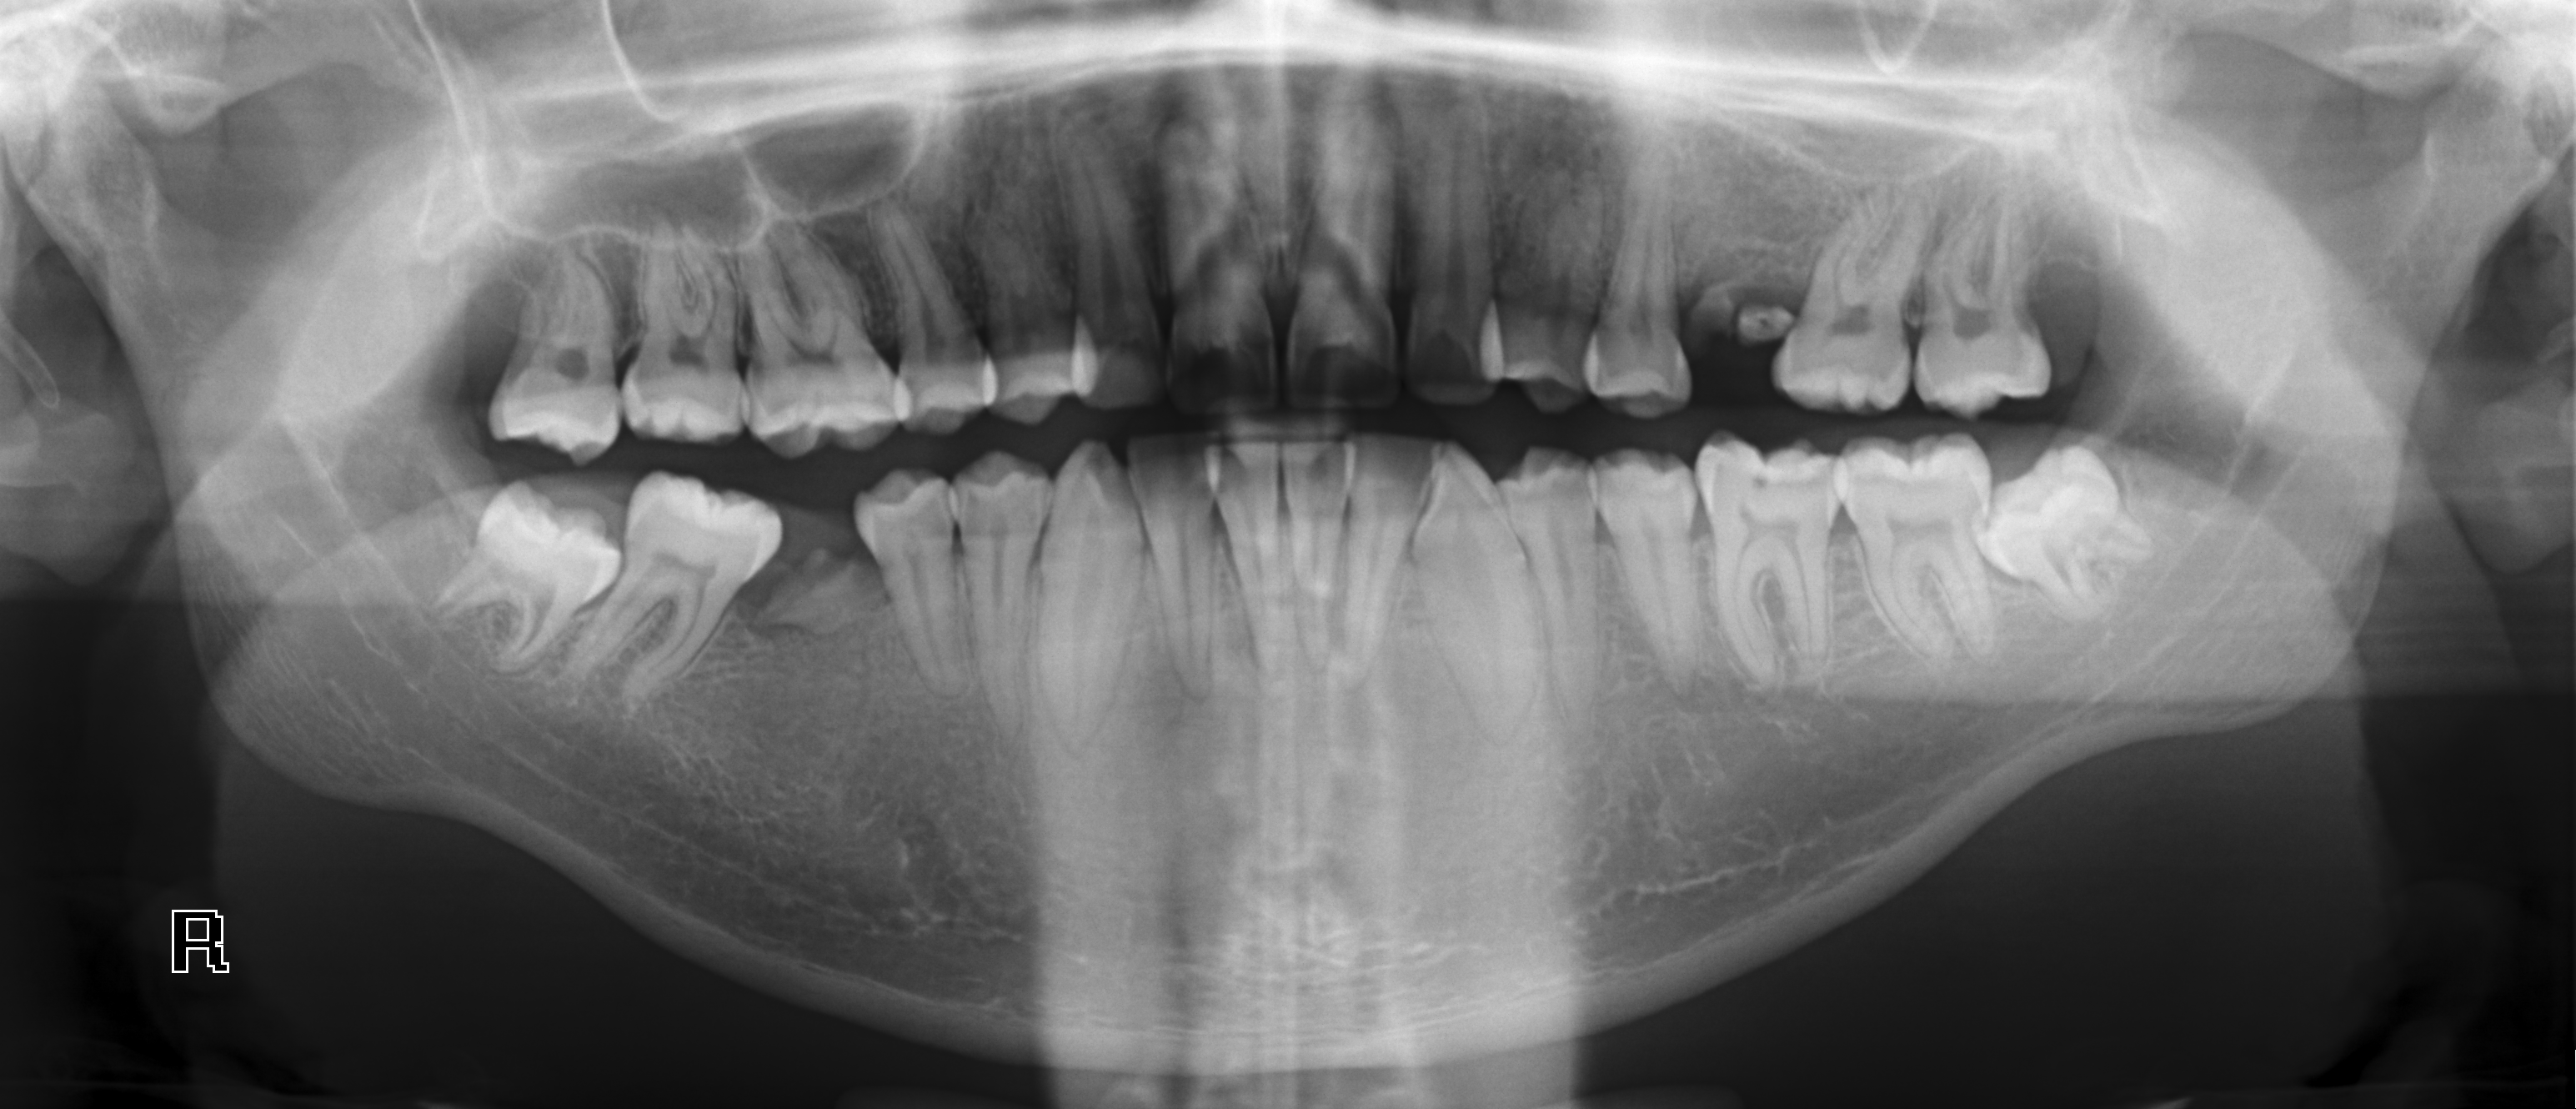
\includegraphics[width=\textwidth]{img/scan.png}
	\caption{Пример тренировочных данных. Томографический снимок}
	\label{fig:scan}
\end{figure}

\begin{figure}[H]
	\centering
	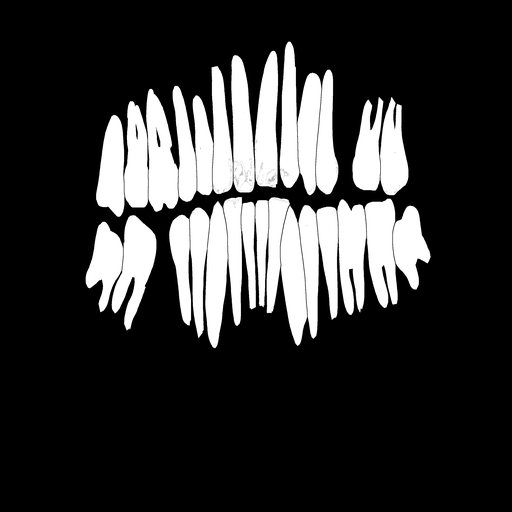
\includegraphics[width=190px]{img/teeth.png}
	\caption{Пример тренировочных данных. Маска зубов}
	\label{fig:teeth}
\end{figure}

\begin{figure}[H]
	\centering
	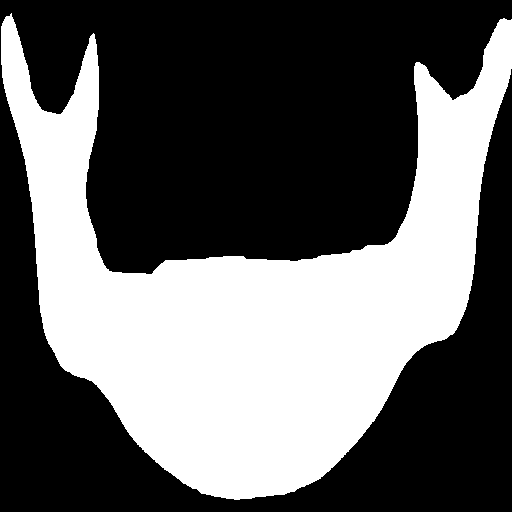
\includegraphics[width=190px]{img/mandible.png}
	\caption{Пример тренировочных данных. Маска нижней челюсти}
	\label{fig:mandible}
\end{figure}

\subsubsection{Классификация зубов при помощи машины опорных векторов}

TODO (допишу в ближайшие пару дней)

\subsubsection{Выделение сегментированных участков}

Для выделения сегментированных (и класифицированных) участков используется метод CCA (от англ. Connected Components Analysis --- анализ связанных компонентов). Данный анализ проводится при помощи выделения на изображений объектов переднего плана (сегментированных участков) и последующего анализа полученного участка. Анализ проводится на основе различных факторов, таких как размер, абсолютное и относительное расположение объекта \cite{cca}.

В листинге \ref{lst:cca} приведена реализация анализа связанных компонентов с их последующим выделением.

\lstinputlisting[
caption={Анализ связанных компонентов},
label={lst:cca},
language=python
]{../../../src/app/cca.py}

На рисунках \ref{fig:segmented} --- \ref{fig:segmented_cca} представлены изображения с выделенными сегментированными участками.

\begin{figure}[H]
	\centering
	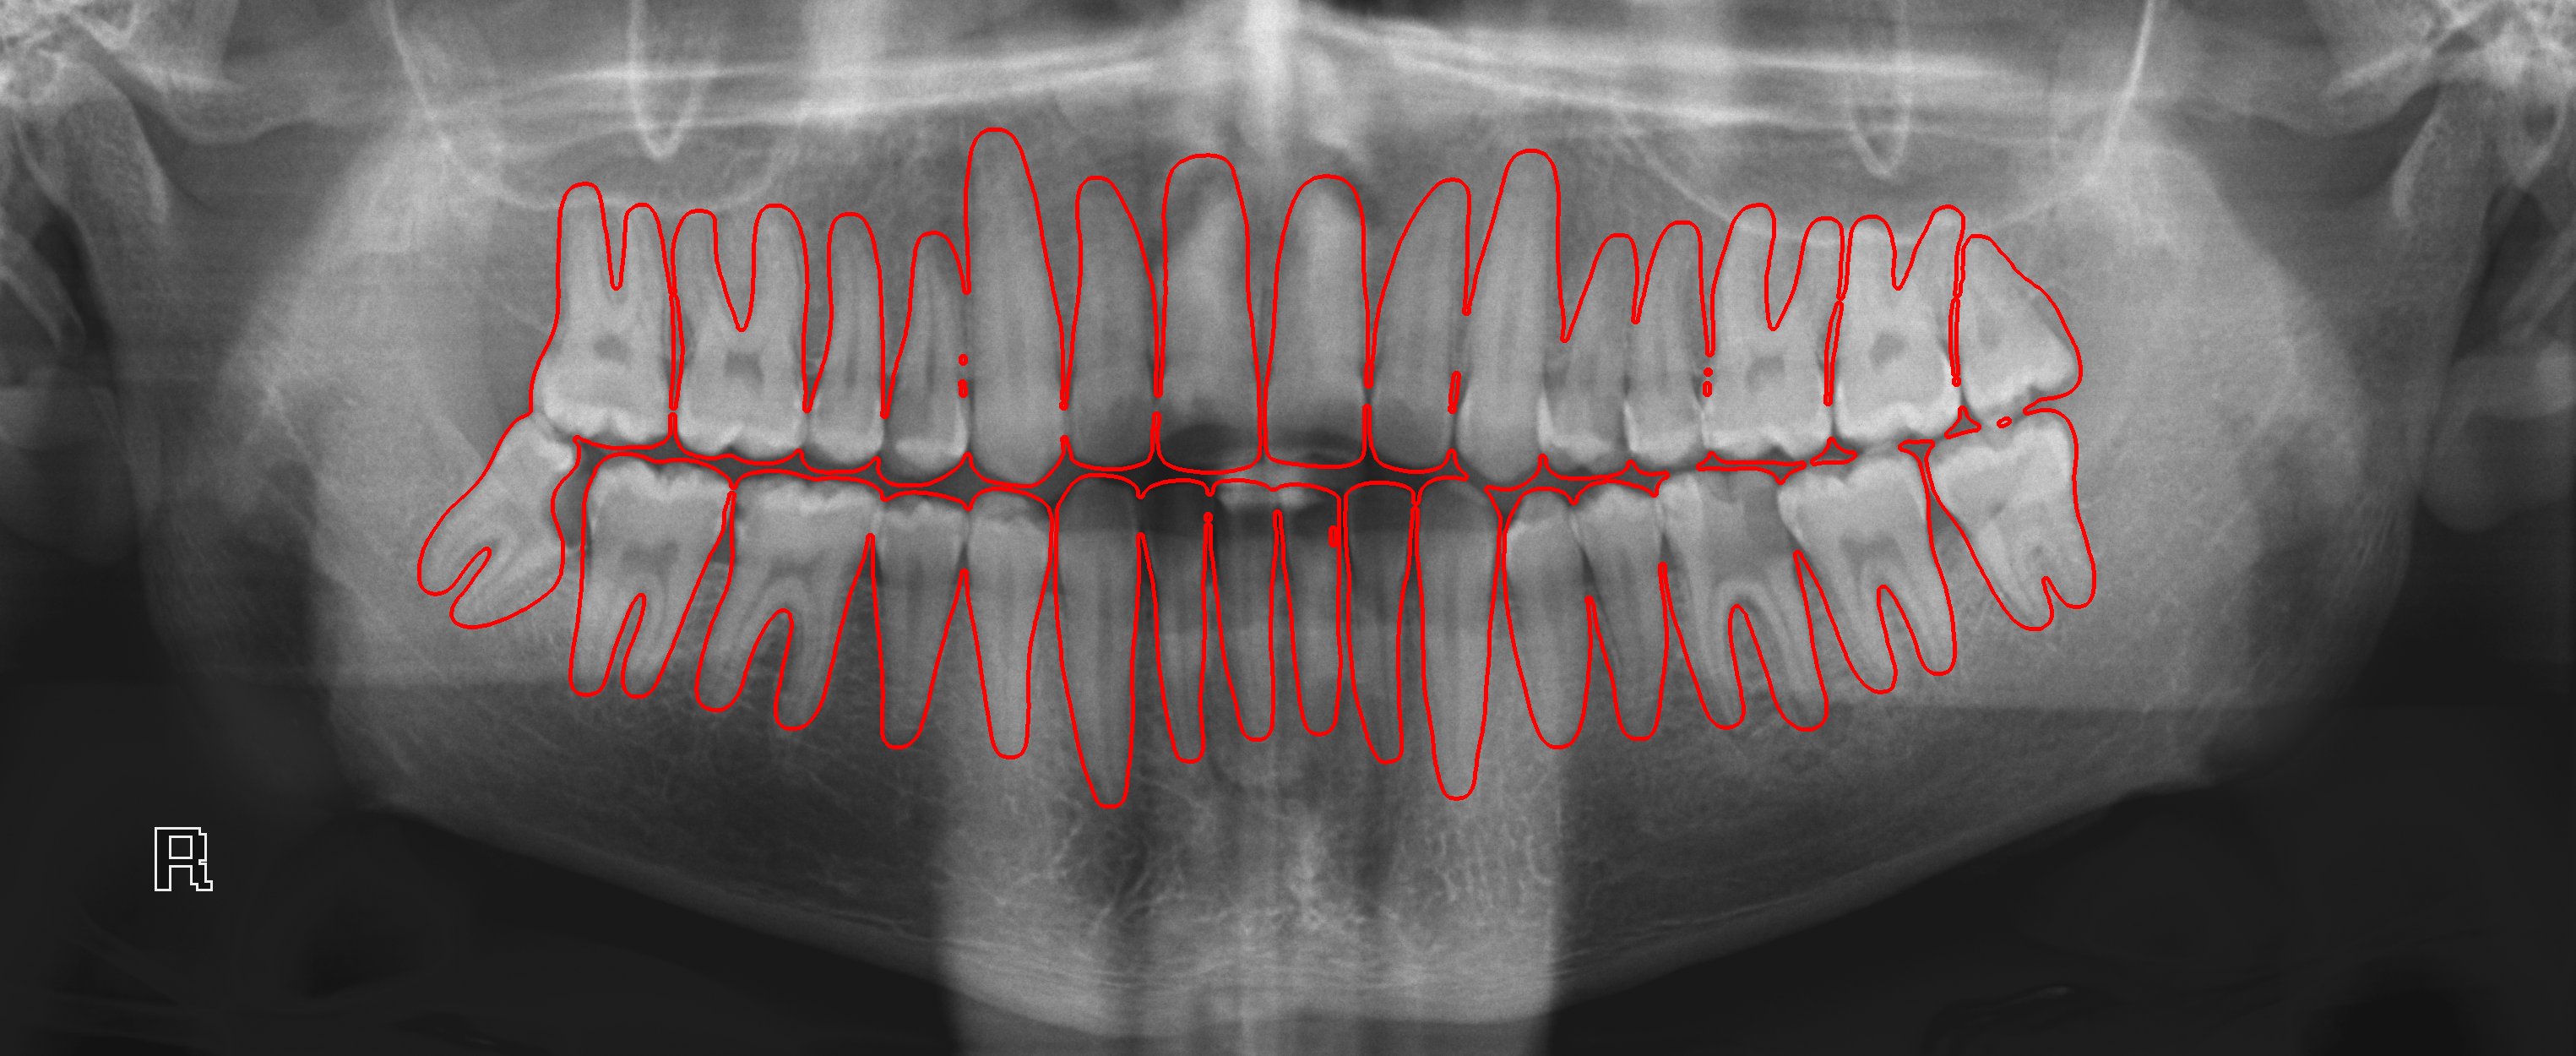
\includegraphics[width=400px]{img/segmented.png}
	\caption{Результат работы семантической сегментации}
	\label{fig:segmented}
\end{figure}

\begin{figure}[H]
	\centering
	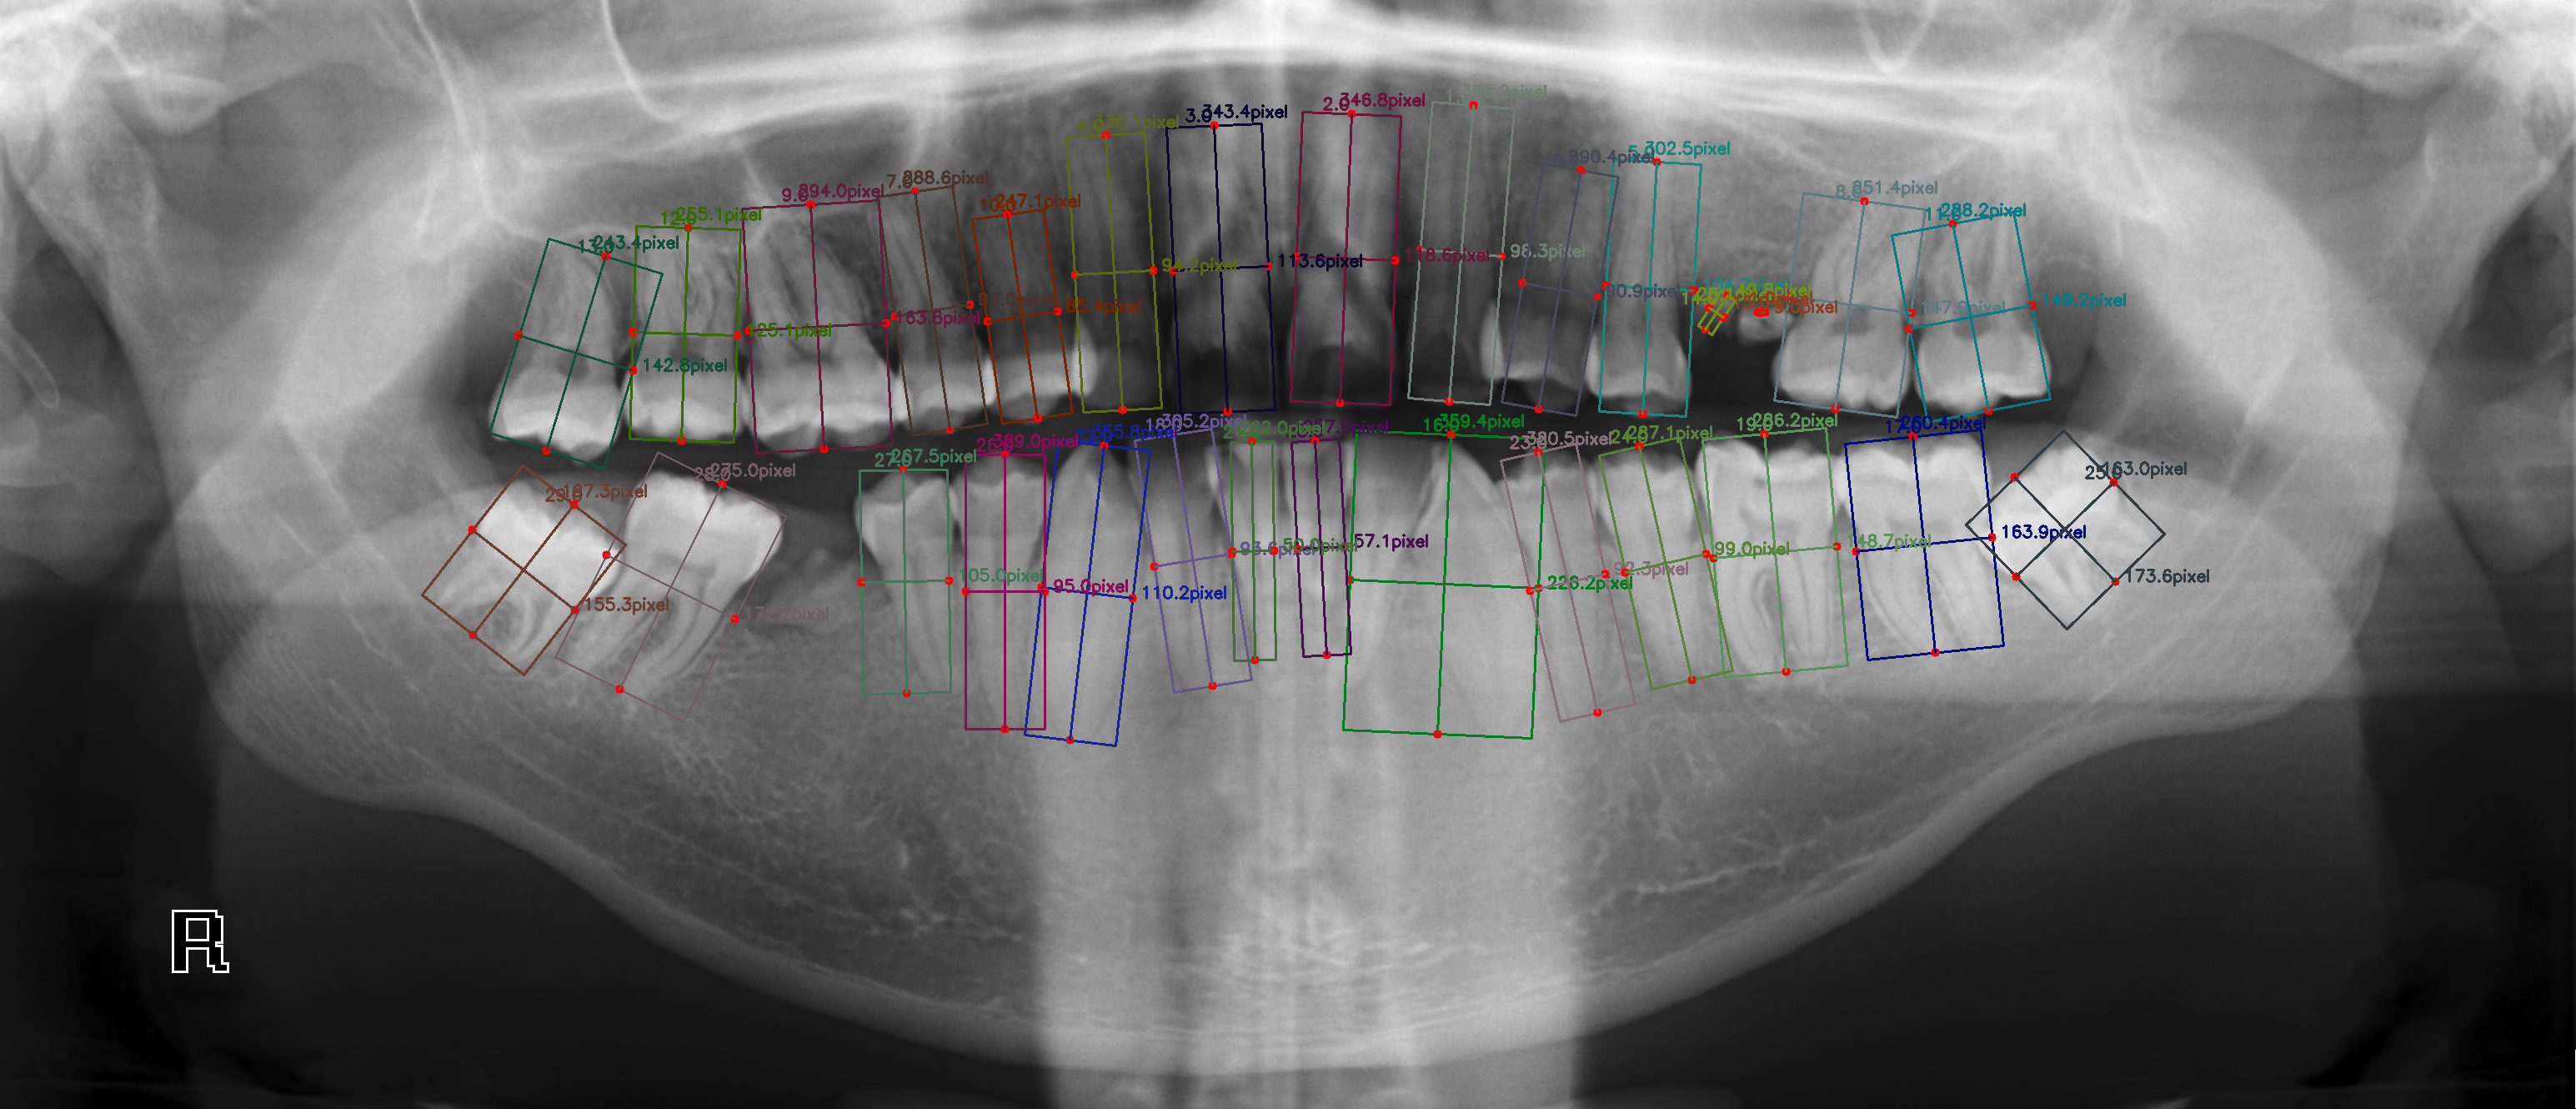
\includegraphics[width=400px]{img/segmented_cca.png}
	\caption{Результат работы сегментации экземпляров}
	\label{fig:segmented_cca}
\end{figure}

\subsection{Результаты обучения модели}

TODO (ждем когда дотренится чтоб графики выдать)

\subsection*{Вывод}

Были описаны средства реализации программного комплекса. Приведены листинги реализации каждого компонента комплекса, примеры работы компонентов, их входные и выходные данные. Описаны технологии и методы, использовавшиеся при реализации.